\documentclass[12pt]{article}
\usepackage{amsmath}
\usepackage{amssymb}
\usepackage{amsthm}
\usepackage{accents}
\usepackage{graphicx}
\setlength{\oddsidemargin}{0in}
\setlength{\textwidth}{6.5in}
\setlength{\topmargin}{-.55in}
\setlength{\textheight}{9in}
\pagestyle{empty}
\renewcommand \d{\displaystyle}
\begin{document}
\noindent Dallas Klumpe

\noindent Math 5820

\noindent Take Home Exam 2

1. A manager believes that experience is the most important factor for a salesperson. To examine this belief, she records last month’s sales (in \$1000s) and the years of experience of 10 randomly selected salespeople. Use the data to:\\
a. Draw a scatter diagram of the data. Here the $x-$axis is the years of experience and the $y-$axis is the sales in $\$1000$.
\begin{center}
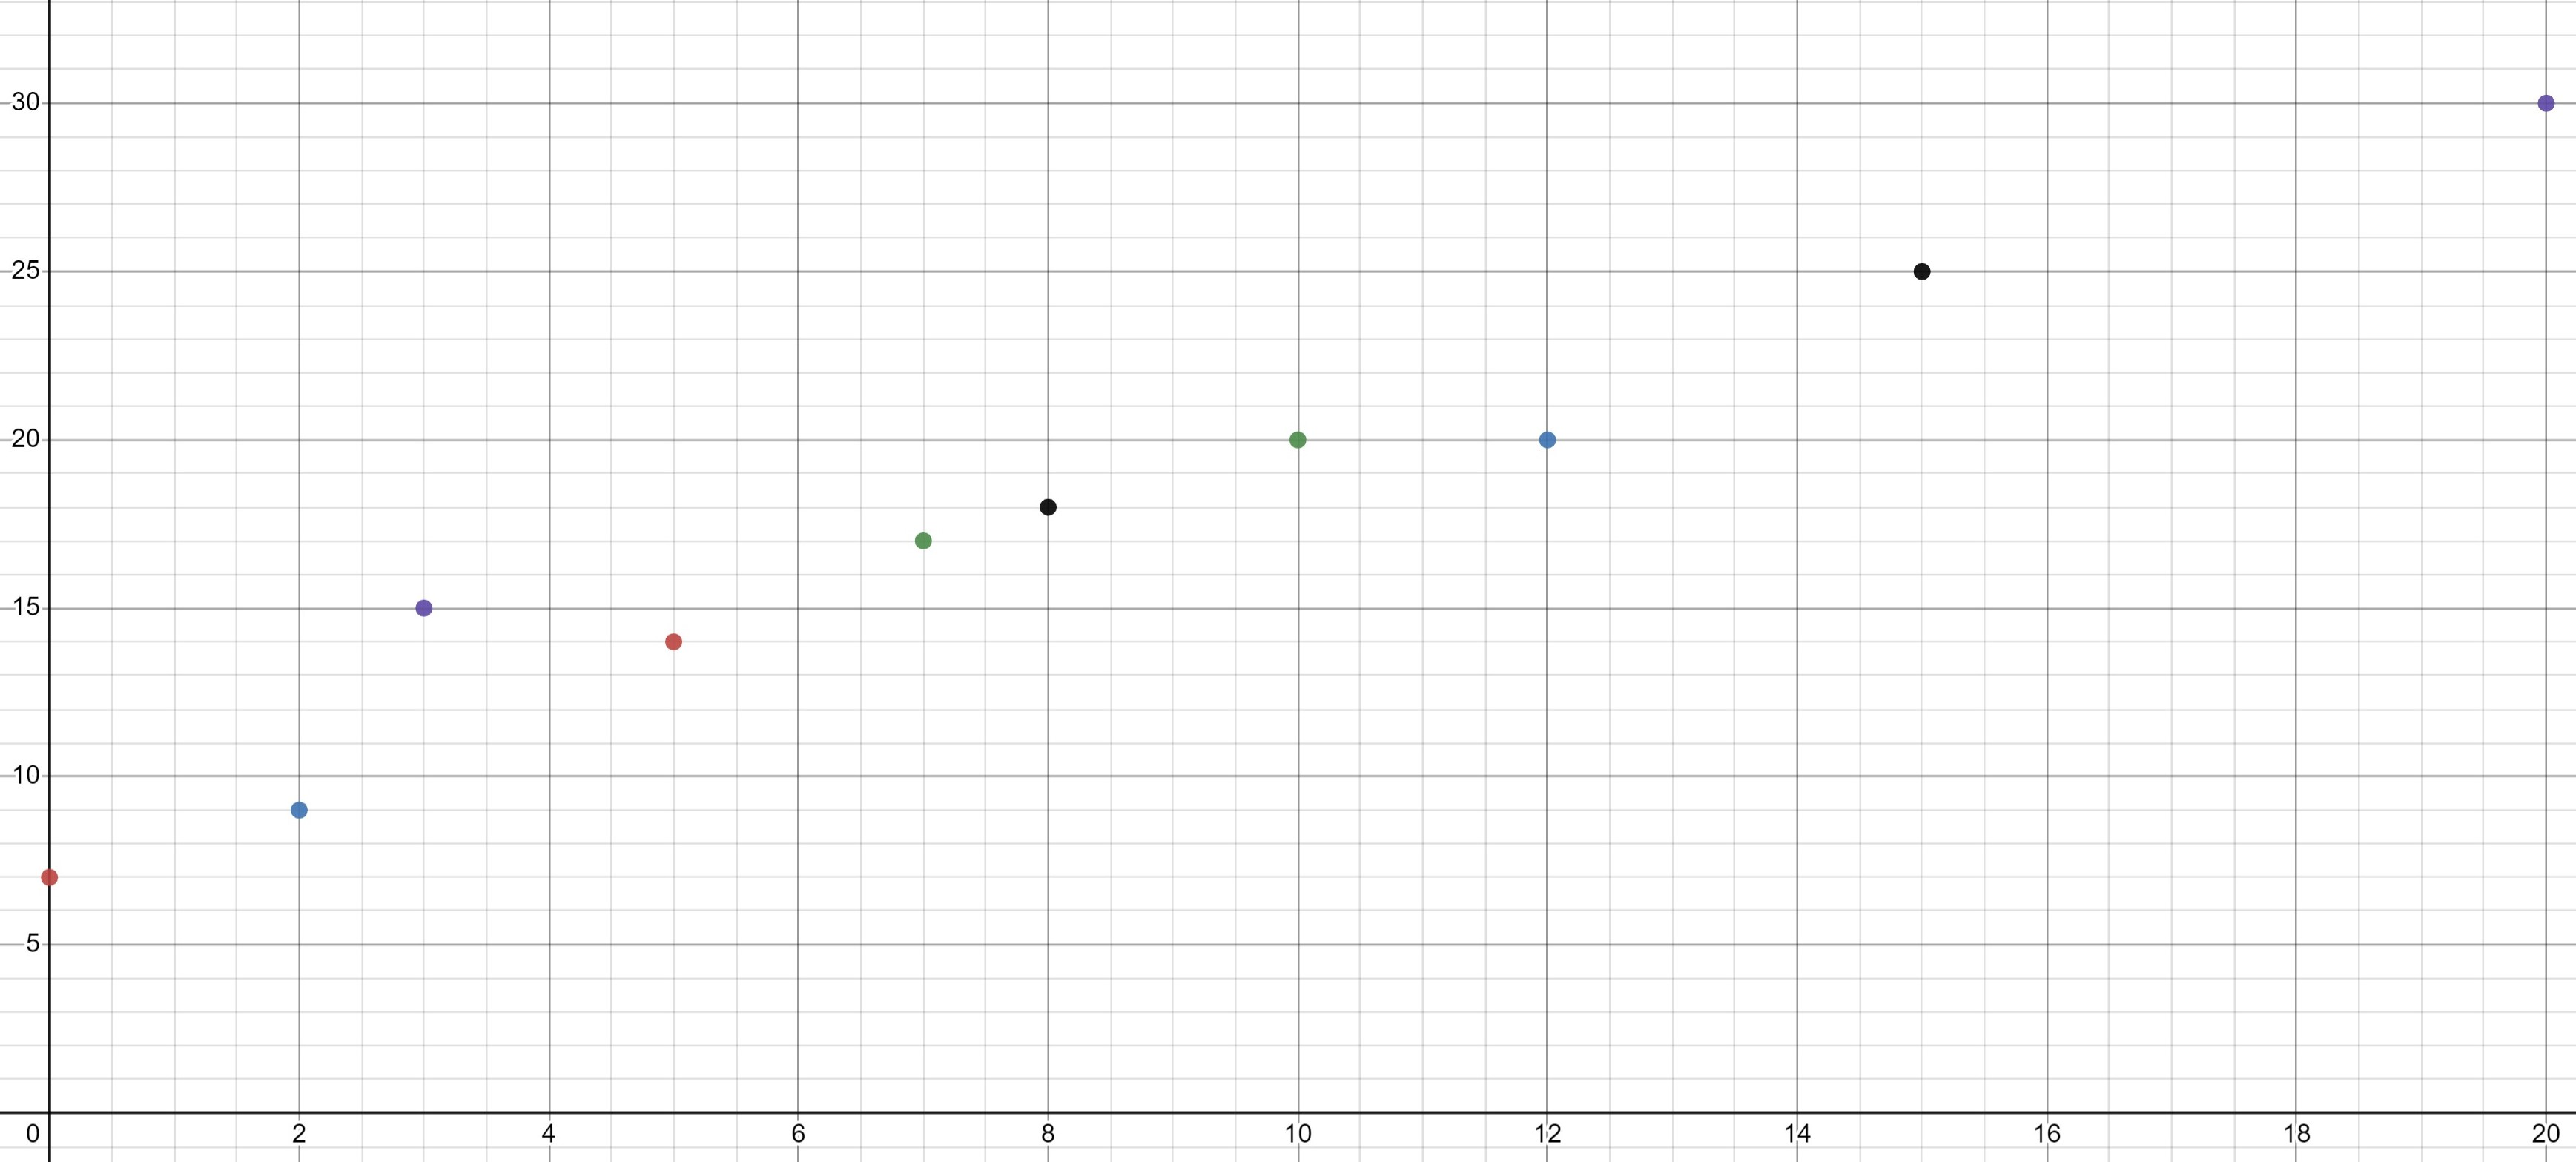
\includegraphics[scale=0.5]{scatplot.JPG}
\end{center}
b. Find the least square regression line.\\
Well, the data gives us $\bar{x}=8.2$ and $\bar{y}=17.5$. Also, $S_{xx}=347.6$ and $S_{xy}=376$. Hence, $\hat{\beta}_1=\frac{S_{xy}}{S_{xx}}=1.0817$ and $\hat{\beta}_0=\bar{y}-\hat{\beta}_1\bar{x}=8.63$.\\
c. Construct a two sided test of $\beta_1$ at the $5\%$ level.\\
Now, $n=10$ and $\alpha=0.05$. So $t_{\alpha/2}=2.306$. By the data, we have that $\sum_{i=1}^10e_i^2=19.7796$ and hence $S^2=\frac{19.7796}{8}=2.4725$. Therefore, our confidence interval is $[\hat{\beta}_1-t_{\alpha/2}\frac{S}{\sqrt{S_{xx}}}, \hat{\beta}_1+t_{\alpha/2}\frac{S}{\sqrt{S_{xx}}}]=[1.0817-2.306(\frac{\sqrt{2.4725}}{\sqrt{347.6}}), 1.0817+2.306(\frac{\sqrt{2.4725}}{\sqrt{347.6}})]=[0.8872, 1.2762]$.\\
d. Determine the sample correlation coefficient $R$ and construct a two sided test for $\rho$ at the $5\%$ level.\\
From the data, we have that $S_{yy}=426.5$. So, $R=\frac{S_{xy}}{\sqrt{S_{xx}S_{yy}}}=\frac{376}{\sqrt{347.6*426.5}}=0.9765$ is our sample correlation coeffiecient. Now we will test $H_0:\rho=0$ versus $H_1:\rho\neq1$ at the $5\%$ level. Well, $t_{\alpha/2}=2.306$. Now, $t=\frac{R\sqrt{n-2}}{\sqrt{1-R^2}}=\frac{0.9765*\sqrt{8}}{\sqrt{1-0.9536}}=12.8258$. Since $t>t_{\alpha/2}$, we reject $H_0$.\\
e. Predict with $95\%$ the mean sales $E(Y|X=9)$ who has 9 years of experiance.\\
Well at $x=9$, $\hat{y}=1.0817(9)+8.63=18.3653$. So, we have a $95\%$ confidence interval of $[18.3653-2.306*\sqrt{2.4725}\sqrt{\frac{1}{10}+\frac{(9-8.2)^2}{347.6}}, 18.3653+2.306*\sqrt{2.4725}\sqrt{\frac{1}{10}+\frac{(9-8.2)^2}{347.6}}]=[17.2082, 19.5224]$. So, the mean sales of a worker who has 9 years of experience is in the interval $[17.2082, 19.5224]$.\\[20pt]

2.  Given the following data drawn from three normal populations:\\
a. Test at the $1\%$ level that the population means of all 3 groups are the same.\\
We will test $H_0:\mu_1=\mu_2=\mu_3$ versus $H_1:$not all $\mu_i$ are equal. We have $\alpha=0.01, k=3$ and $n=5+6+4=15$. Now, our ANOVA table is:
\begin{center}
\begin{tabular}{ c|   c   c   c   c  }
Source & df & SS & MS & F\\
\hline
Treatment & 2 & 46.9333 & 23.4667 & 3.2\\
Error & 12 & 88 & 7.3333 & \\
Total & 14 & 134.933 &  & 
\end{tabular}
\end{center}
So, $F=3.2$. Now, $F_{\alpha}=0.01$ and $F_{1-\alpha}=6.93$. Since $F_{\alpha}<F<F_{1-\alpha}$, we fail to reject $H_0$. If $\alpha=0.1$, we have $F_{\alpha}=0.106$ and $F_{1-\alpha}=2.81$ and we would reject the null hypothesis.
b. Construct $95\%$ Tukey's and Fisher's intervals to test the pariwise subhypothesis of the 3 groups.\\
\textbf{Tukey}: We have $\alpha=0.05, r=\frac{3}{\frac15+\frac16+\frac14}=4.8649\approx5, \bar{y}_1=12, \bar{y}_2=12$, and $\bar{y}_3=16$. Then, $Q_{\alpha}=3.77$ and $D=\frac{3.77}{\sqrt{4.8649}}=1.7093$. So, our general Tukey interval will be $[(\bar{y}_i-\bar{y}_j)-1.7093\sqrt{7.3333}, (\bar{y}_i-\bar{y}_j)+1.7093\sqrt{7.3333})]$. Then we have the following table:
\begin{center}
\begin{tabular}{ c   c   c  }
$\mu_1-\mu_2$ & [-4.6288, 4.6288] & fail to reject\\
$\mu_1-\mu_3$ & [-8.6288, 0.6288] & fail to reject\\
$\mu_2-\mu_3$ & [-8.6288, 0.6288] & fail to reject
\end{tabular}
\end{center}
So, we fail to reject all means being equal.\\
\textbf{Fisher}: Using the same data, we have that $t_{\alpha/2}=2.1788$. So our general Fisher interval is $[(\bar{y}_i-\bar{y}_j)-2.1788\sqrt{7.3333(\frac{1}{n_i}+\frac{1}{n_j})}, (\bar{y}_i-\bar{y}_j)+2.1788\sqrt{7.3333(\frac{1}{n_i}+\frac{1}{n_j})}]$. Thus, we have the following pairwise table:
\begin{center}
\begin{tabular}{ c   c   c  }
$\mu_1-\mu_2$ & [-2.2532, 2.2532] & fail to reject\\
$\mu_1-\mu_3$ & [-6.2532, -1.7468] & reject\\
$\mu_2-\mu_3$ & [-6.2532, -1.7468] & reject
\end{tabular}
\end{center}
Hence, we reject $\mu_1=\mu_3$ and $\mu_2=\mu_3$.\\[20pt]

3.a. Let $\hat{\beta}_0$ and $\hat{\beta}_1$ be the least square estimators for $\beta_0$ and $\beta_1$. Show that Cov$(\hat{\beta}_0,\hat{\beta}_1)=-\frac{\bar{X}\sigma^2}{S_{xx}}$.\\
Well, Cov$(\hat{\beta}_0, \hat{\beta}_1)=E((\hat{\beta}_0-E(\hat{\beta}_0))(\hat{\beta}_1-E(\hat{\beta}_1)))=E((\hat{\beta}_0-\beta_0)(\hat{\beta}_1-\beta_1))=E(\bar{y}-(\hat{\beta}_1-\beta_1)\bar{X}(\hat{\beta}_1-\beta_1))=E(\bar{Y}(\hat{\beta}_1-\beta_1)-\bar{X}(\hat{\beta}_1-\beta_1)^2)=0-\bar{X}E(\hat{\beta}_1-\beta_1)^2=-\bar{X}$Var$(\beta_1)=-\frac{\bar{X}\sigma^2}{S_{xx}}$ as desired.\\
b. Using (a), show that Cov$(\bar{Y},\hat{\beta}_1)=0$.\\
Well, Cov$(\bar{Y},\hat{\beta}_1)=$Cov$(\sum_{i=1}^nY_i,\sum_{j=1}^n\frac{S_{xy}}{S_{xx}})=\sum_{i=1}^n\frac{(x_i-\bar{x})\sigma^2}{nS_{xx}}$Cov$(Y_i,Y_j)=0$ as desired.%E(\bar{Y}\hat{\beta}_1)-E(\bar{Y}-E(\bar{Y}))(\hat{\beta}_1-\beta_1)=E(\bar{Y}-\bar{Y})(\hat{\beta}_1-\beta_1)=0$ as desired.





\end{document}